
\chapter{Test d'intégration}

Nous n'avons malheureusement pas pu faire de nombreux tests d'intégrations puisque à la fin de notre projet nous n'avions pas la totalité des composants pour monter notre radiogoniomètre. Néanmoins nous avons pu tester l'intégration du radiogoniomètre au \rpi en plaçant des leds sur les ports GPIO, ainsi que l'intégration de l'application mobile au serveur central.


\section{Raspberry Pi}
La documentation technique lié a notre Raspberry Pi es situé en annexe à la page \pageref{annexe:rpi}
~\\

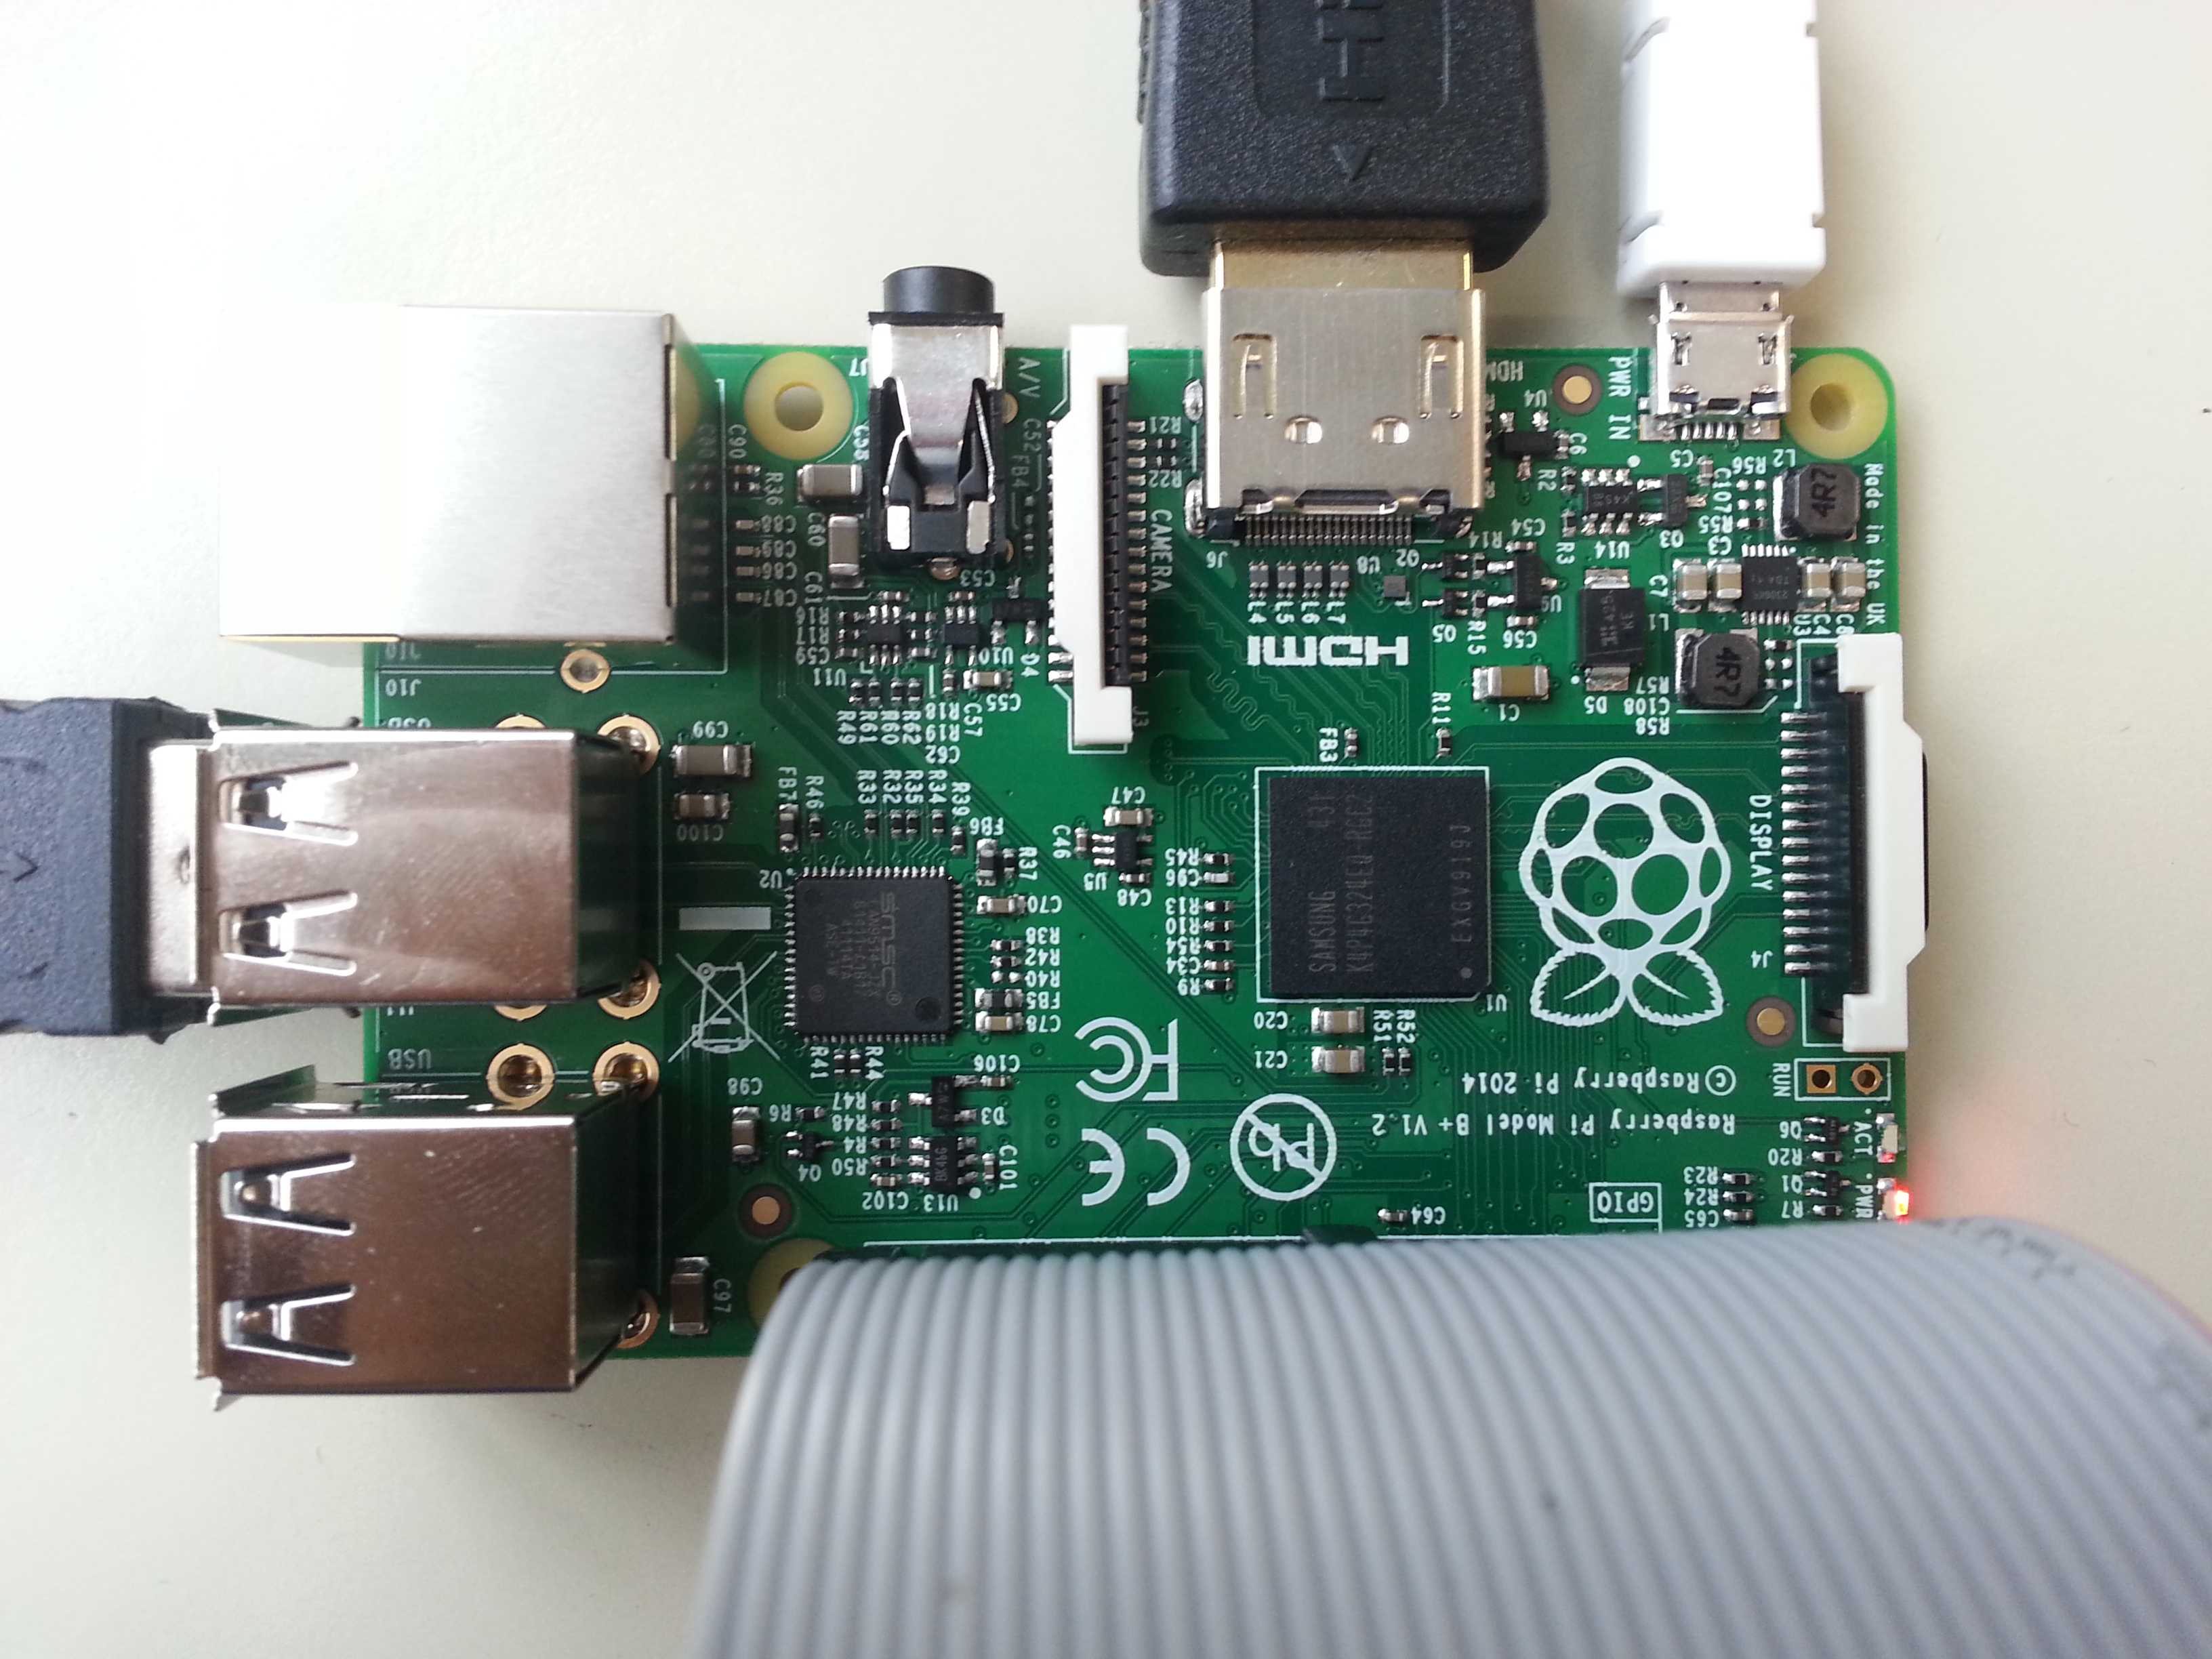
\includegraphics[width=\textwidth]{Test_unitaire/Rpi/img5.jpg}
\captionof{figure}{Notre Raspberry Pi B+}

~\\
\parindent=15pt

Pour s'assurer que notre Raspberry Pi répond aux spécifications fonctionnelles et qu'il fonctionne correctement en toutes circonstances pour notre projet, nous y avons réalisé des tests intégrations.

Après avoir enfin installé le système d'exploitation Raspbian\footnote{La documentation lié à Raspbian est situé en annexe à la page \pageref{annexe:raspbian}} sur notre Raspberry Pi B+, nous avons tenté de tester les ports GPIO. Pour cela, dans un premier temps, nous avons allumé des LED grâce à un script python à travers différents ports GPIO. Sur la figure \ref{figure:led}, on peut observer que nous avons allumé une LED grâce au port 22.
~\\

Dans notre projet le Raspberry Pi sera placé entre le radio-goniomètre à effet Doppler et l'utilisateur. Il aura deux taches, corréler les données entre tous les dispositifs pour obtenir la position du drone et afficher le résultat à l'utilisateur. Pour cela il doit récupérer la direction qui est donné par le Montréal 3v2. Cette position est donnée à travers des LED (voir figure \ref{figure:ledMontreal}). Nous allons donc placer le Raspberry Pi au niveau des LED pour obtenir les informations délivré par le Montréal 3v2. % TODO : A FINIR

\begin{figure}[!h]
  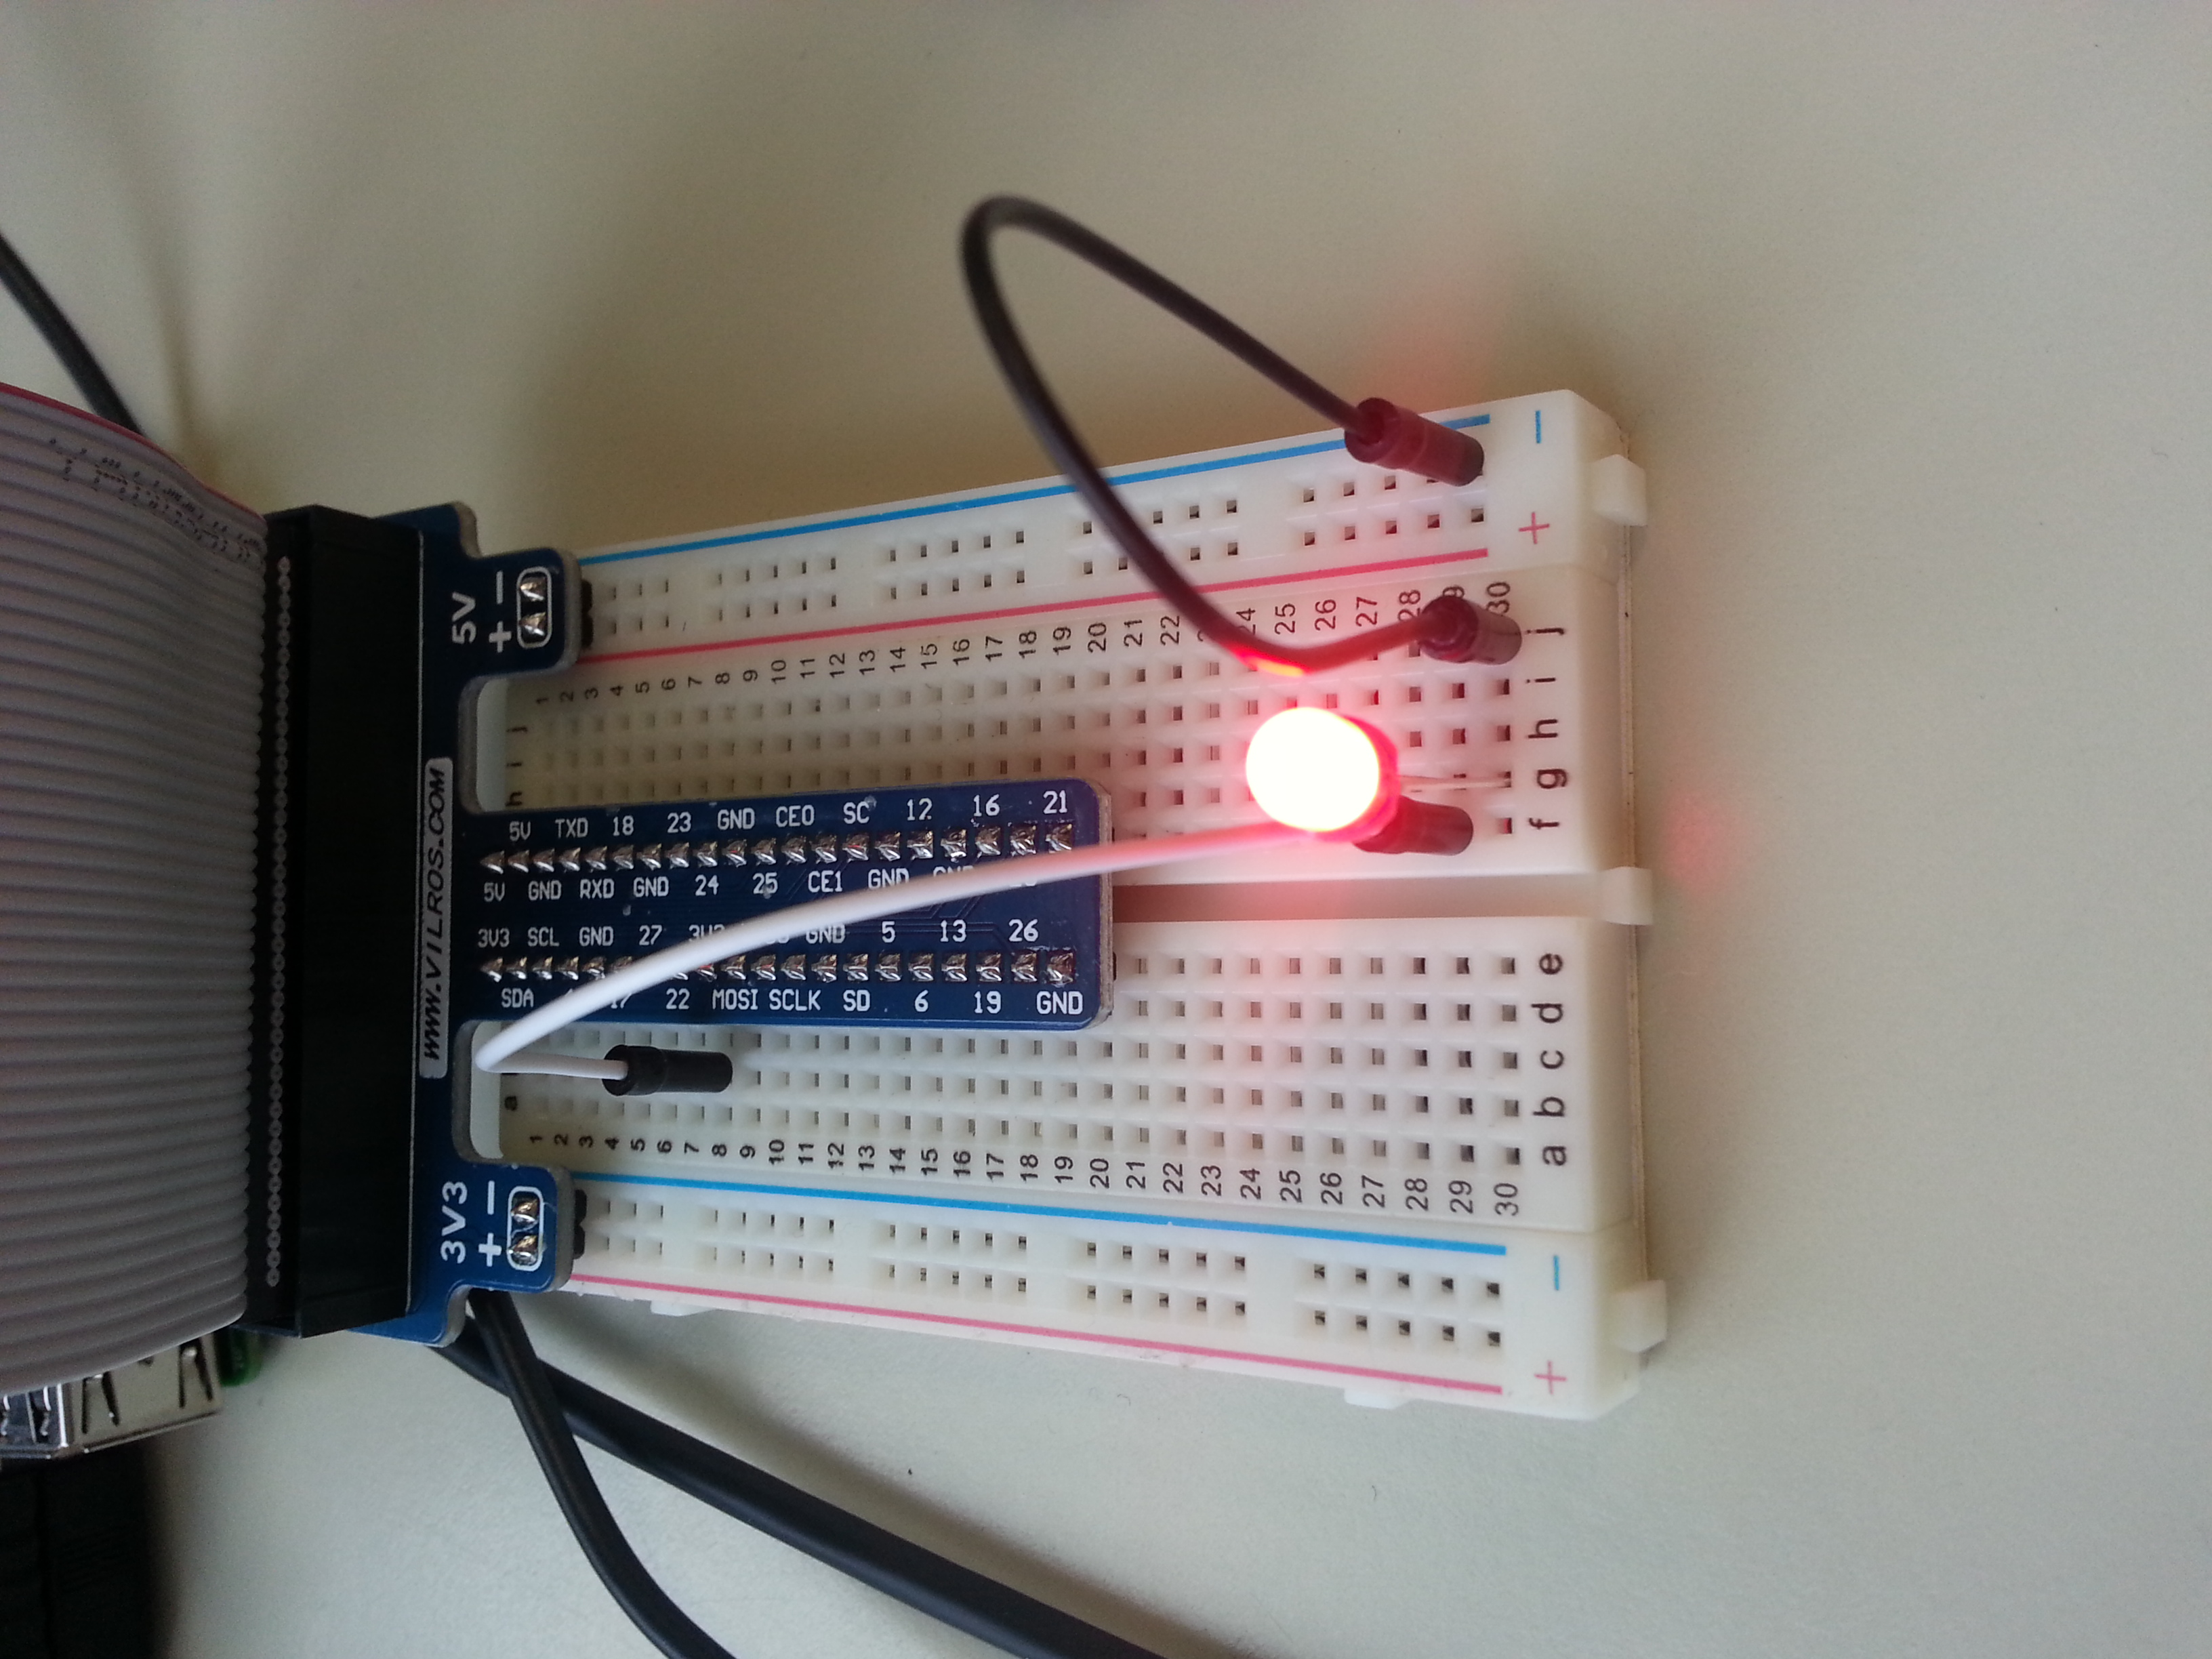
\includegraphics[width=\textwidth]{Test_unitaire/Rpi/img3.jpg}
  \caption{Allumage d'une LED par Raspberry Pi}
  \label{figure:led}
\end{figure}

\begin{figure}[!h]
  \centering
  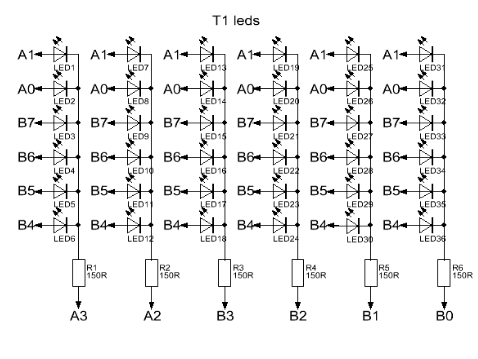
\includegraphics[width=0.8\textwidth]{Test_unitaire/Rpi/led.png}
  \caption{Méthode de connexion des leds dans le Montréal}  
  \label{figure:ledMontreal}
\end{figure}
\begin{figure}[!h]
  \centering
  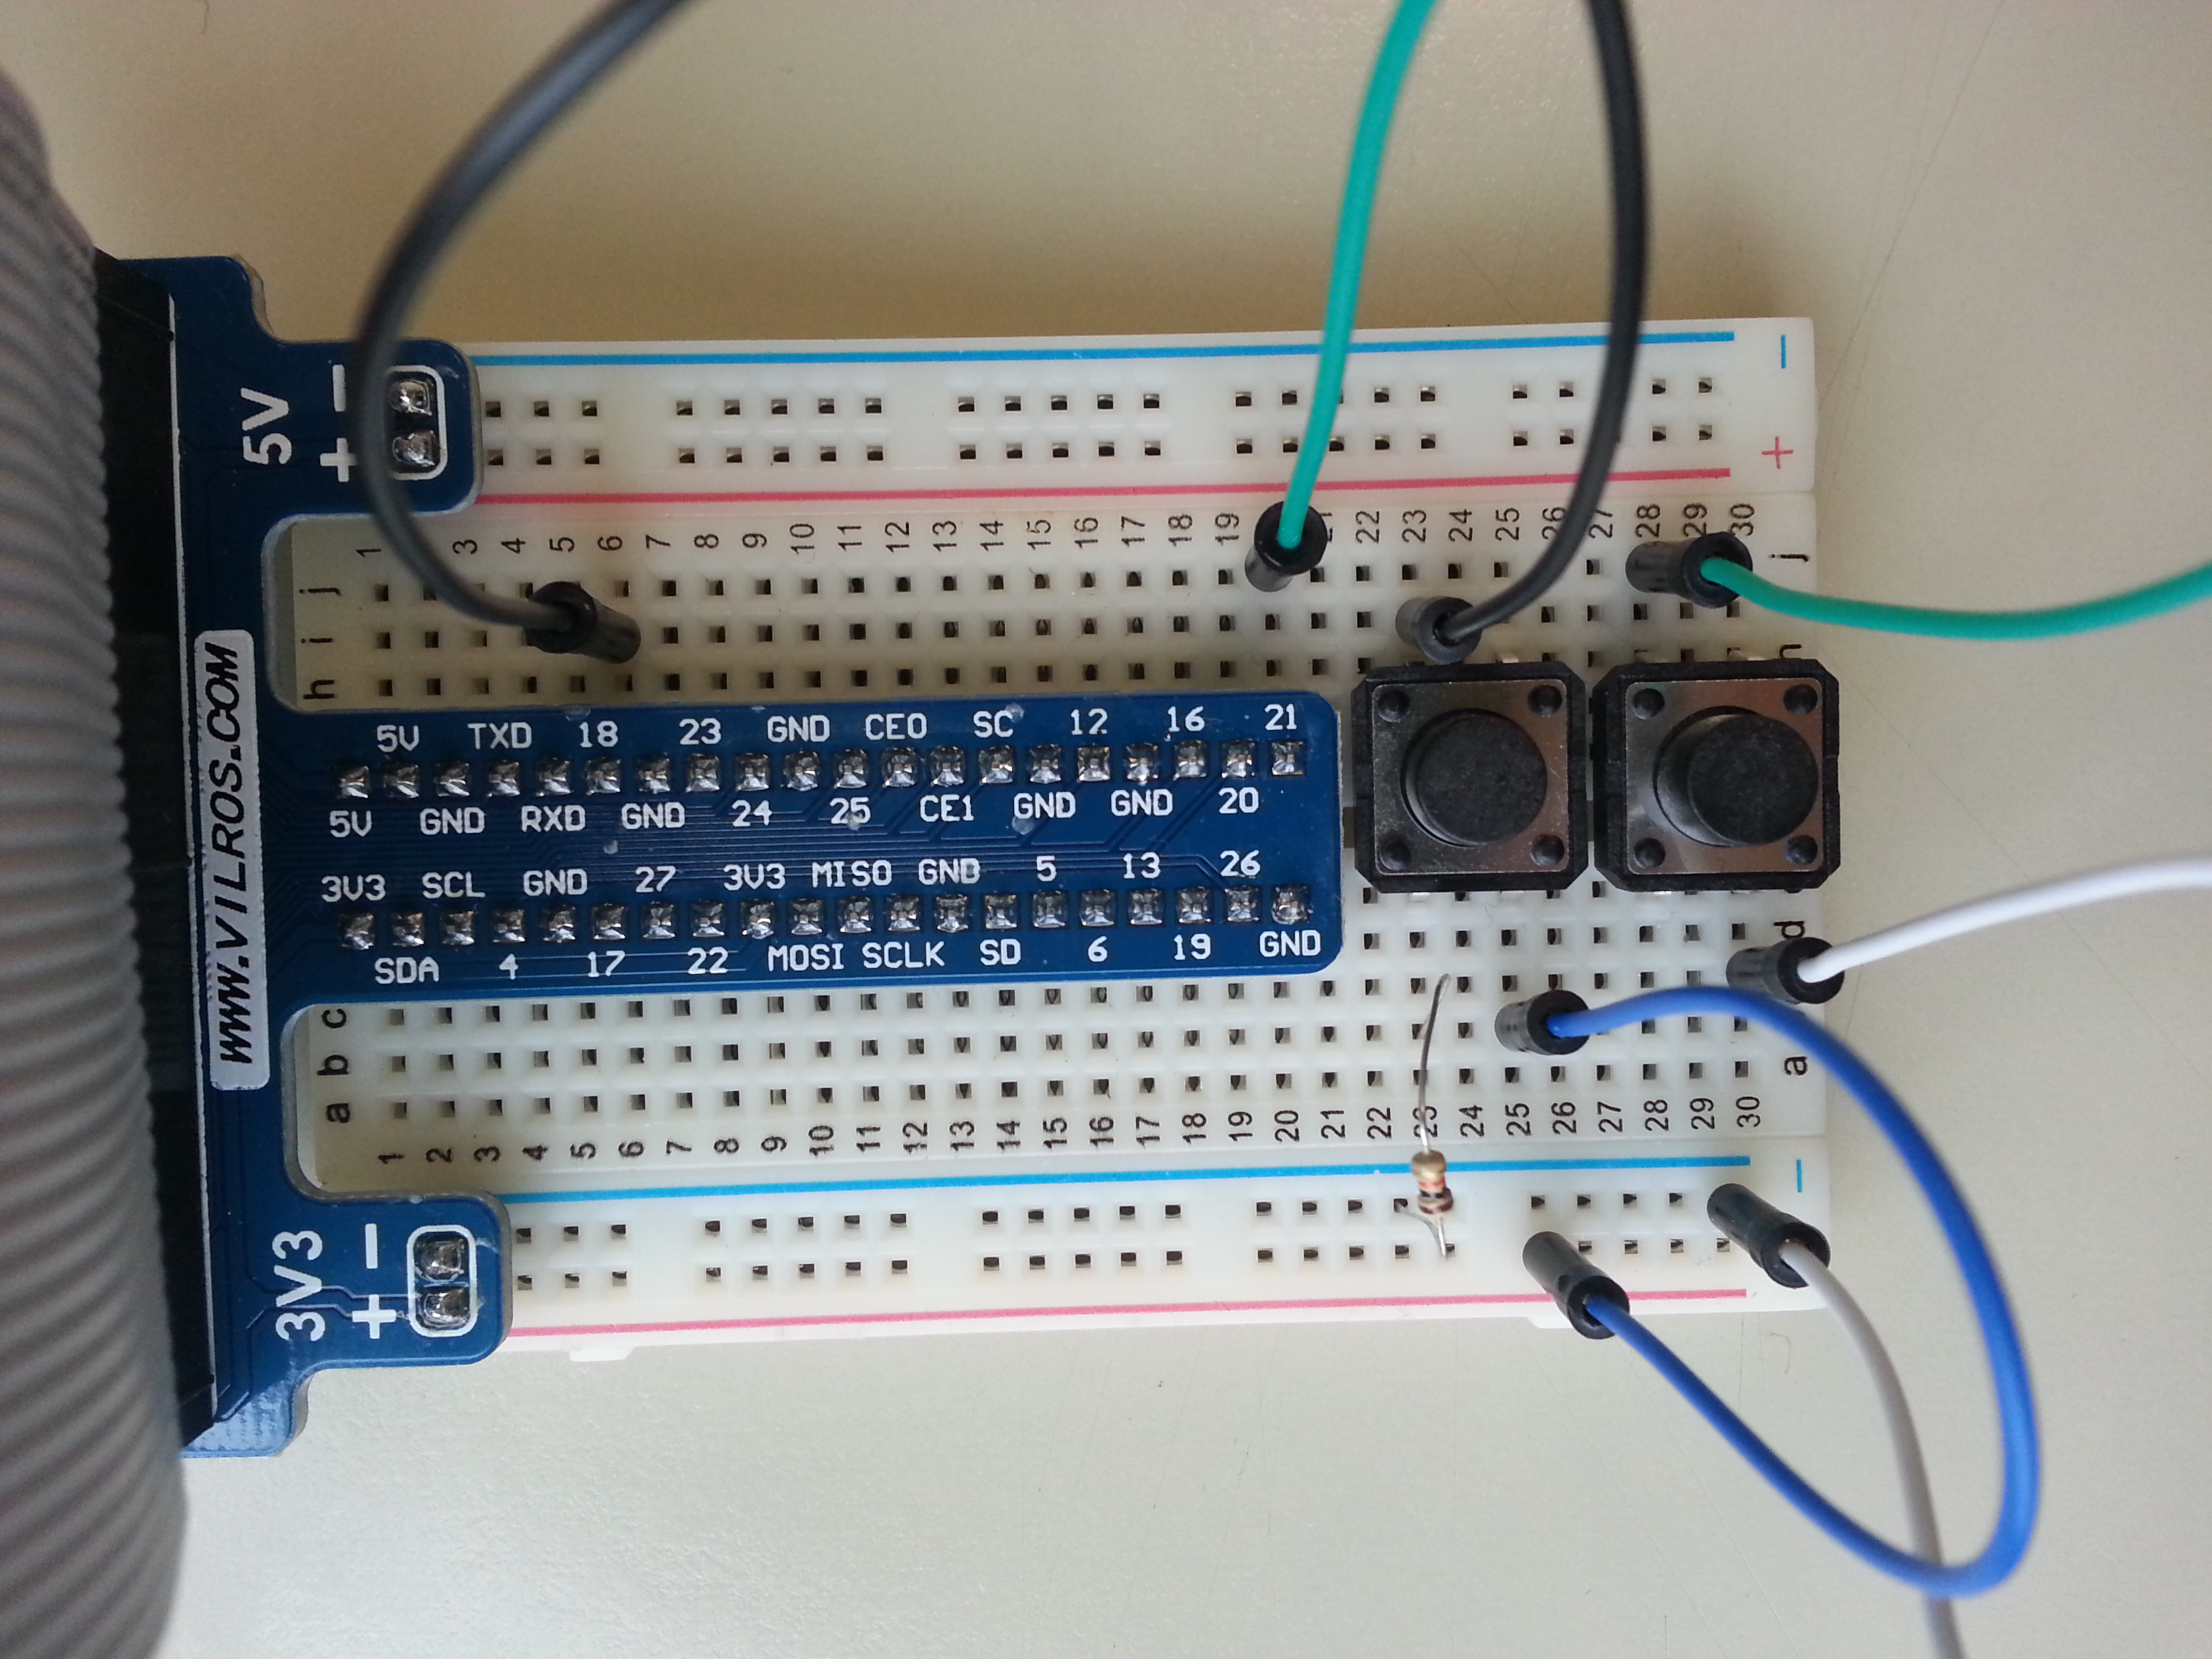
\includegraphics[width=\textwidth]{Test_unitaire/Rpi/img4.jpg}  
  \caption{Système modélisant une LED}
  \label{figure:test}
\end{figure}

La sortie du Montréal 3v2 est décrite à la figure \ref{figure:ledMontreal}. On constate que le pic qui permet l'affichage à 12 sortie qui lui permet de gérer 24 LED. Pour connaître quelle LED est allumé, il faut savoir laquelle des entré A1,A0,B7,B6,B5,B4 à un front montant et laquelle des entrées B0,B1,B2,B3,A3,A2 à un front descendant.

Pour modéliser une LED en entré du Raspberry Pi, nous avons positionné 2 boutons poussoirs (voir figure \ref{figure:test}). Le premier permets de réaliser le front montant et le second le front descendant. Ainsi en positionnant ces boutons au bon endroit par rapport au port GPIO du raspberry il est possible de connaître quelle LED on a simuler.

Nous avons réaliser un script python qui lié les entrées du raspberry avec les sortie du pic. Puis nous avons tester en simulant une LED comme décrit précédemment.

On peut constater que l'expérience est un succès car le raspberry pi nous renvoie bien le numéro de la LED que nous voulions tester.


\section{Android}

Les tests d'intégration de l'application android ont été réalisé au cour de notre projet. Pour cela nous avons envoyé des chaînes de caractères du serveur vers l'application android et nous avons vérifié leur réception.



%%% Local Variables: 
%%% mode: latex
%%% TeX-master: "../rapport"
%%% End: 